\documentclass[aspectratio=169,10pt]{beamer}

% --- Theme and Styling Configuration ---
\usetheme{Madrid}
\usecolortheme{whale}

% Typography and Layout Packages
\usepackage{booktabs}
\usepackage{tabularx}
\usepackage{multirow}
\usepackage{amsmath,amssymb}
\usepackage{tcolorbox}
\usepackage{tikz}
\usetikzlibrary{arrows.meta,positioning,shapes.geometric,fit,backgrounds,calc}

% Define Educational Knowledge Graph Color Palette
\definecolor{primaryblue}{RGB}{20, 52, 100}
\definecolor{accentteal}{RGB}{0, 150, 136}
\definecolor{darkslate}{RGB}{33, 43, 54}
\definecolor{lightgraybg}{RGB}{245, 247, 250}
\definecolor{warnred}{RGB}{198, 40, 40}
\definecolor{successgreen}{RGB}{46, 125, 50}

\setbeamercolor{palette primary}{bg=primaryblue,fg=white}
\setbeamercolor{palette secondary}{bg=accentteal,fg=white}
\setbeamercolor{palette tertiary}{bg=primaryblue!80,fg=white}
\setbeamercolor{structure}{fg=primaryblue}
\setbeamercolor{title}{fg=white,bg=primaryblue}
\setbeamercolor{frametitle}{fg=white,bg=primaryblue}
\setbeamercolor{block title}{bg=primaryblue!15,fg=primaryblue}
\setbeamercolor{block body}{bg=lightgraybg,fg=darkslate}
\setbeamercolor{block title alerted}{bg=warnred!15,fg=warnred}
\setbeamercolor{block body alerted}{bg=lightgraybg,fg=darkslate}
\setbeamercolor{block title example}{bg=accentteal!15,fg=accentteal}
\setbeamercolor{block body example}{bg=lightgraybg,fg=darkslate}

\setbeamertemplate{navigation symbols}{}
\setbeamertemplate{footline}[frame number]

% --- Presentation Metadata ---
\title[Evidence-Grounded Multi-Relation Edu-KG]{Multi-Relation Educational Knowledge Graph Construction and Rigorous Evaluation}
\subtitle{Source-Grounded Extraction, Educational Weighting, and Verification Independence}
\author[LearnKG Framework]{Educational Knowledge Engineering Group}
\institute[LearnKG]{Curriculum AI \& Knowledge Graph Research}
\date{\today}

\begin{document}

% -----------------------------------------------------------------------------
% SLIDE 1: Title Slide
% -----------------------------------------------------------------------------
\begin{frame}[plain]
    \titlepage
\end{frame}

% -----------------------------------------------------------------------------
% SLIDE 2: Core Philosophy & Grounding Paradigm
% -----------------------------------------------------------------------------
\begin{frame}{Core Philosophy: Source-Grounded \& Self-Contained}
    \begin{columns}[T]
        \begin{column}{0.48\textwidth}
            \begin{block}{Independence from External Priors}
                \begin{itemize}
                    \item \textbf{No Wikipedia/Web Hallucinations:} Knowledge graphs often inject ungrounded encyclopedic noise.
                    \item \textbf{Strict In-Text Provenance:} Every concept node and relation triple is bound to verified chapter/page coordinates.
                    \item \textbf{Curriculum Self-Containment:} Learning sequences represent what the target textbook \textit{actually teaches}, not an idealized ontology.
                \end{itemize}
            \end{block}
        \end{column}

        \begin{column}{0.48\textwidth}
            \begin{exampleblock}{The Multi-Stage Evidence Contract}
                \begin{itemize}
                    \item \textbf{Textbook Sentence Anchor:} Every proposal requires a verbatim supporting sentence.
                    \item \textbf{Explicit Typological Boundary:} Formal rejection of category errors (e.g., separating \textit{Type-of} hyponymy from \textit{Part-of} meronymy).
                    \item \textbf{Decoupled Weighting:} Model extraction confidence is never conflated with pedagogical relation weight.
                \end{itemize}
            \end{exampleblock}
        \end{column}
    \end{columns}

    \vspace{0.4cm}
    \begin{tcolorbox}[colback=lightgraybg,colframe=accentteal,title=\textbf{Verification Rule},sharp corners]
        \small An edge is rejected if its supporting quote cannot be mapped verbatim to the textbook corpus or if the direction violates pedagogical dependencies.
    \end{tcolorbox}
\end{frame}

% -----------------------------------------------------------------------------
% SLIDE 3: Dataset Details: CK-12 Basic Geometry
% -----------------------------------------------------------------------------
\begin{frame}{Dataset Characteristics: CK-12 Basic Geometry}
    \begin{columns}[T]
        \begin{column}{0.52\textwidth}
            \begin{block}{Textbook Ingestion \& Corpus Structure}
                \begin{itemize}
                    \item \textbf{Source Corpus:} \texttt{ck12\_basic\_geometry\_concepts.txt}
                    \item \textbf{Structure Blocks:} $72$ hierarchical blocks parsed into $12$ major chapters and $60$ pedagogical modules.
                    \item \textbf{Target Concepts:} $130$ canonical mathematical concepts extracted with definitional grounding.
                    \item \textbf{Reference Benchmark:} AL-CPL Geometry benchmark ($1,681$ annotated gold pairs; $524$ positive prerequisites).
                \end{itemize}
            \end{block}
        \end{column}

        \begin{column}{0.44\textwidth}
            \begin{block}{Textbook Corpus Breakdown}
                \centering
                \footnotesize
                \begin{tabular}{lr}
                    \toprule
                    \textbf{Corpus Dimension} & \textbf{Value} \\
                    \midrule
                    Textbook Chapters & 12 \\
                    Instructional Sections & 60 \\
                    Parsed Concepts ($|V|$) & 130 \\
                    Definitional Sentence Matches & 67 / 130 \\
                    Syntactic Candidates ($O(V^2)$) & 9,372 \\
                    \textbf{Filtered Candidate Pairs} & \textbf{810} \\
                    \textbf{Final Verified Edges ($|E|$)} & \textbf{84} \\
                    \bottomrule
                \end{tabular}
            \end{block}
        \end{column}
    \end{columns}

    \vspace{0.2cm}
    \begin{alertblock}{Eliminating the $O(V^2)$ Cartesian Explosion}
        \footnotesize Combining embedding retrieval, definitional co-mentions, and chapter structure narrows the evaluation set from 9,372 pairs down to 810 grounded candidate pairs with full provenance tracking.
    \end{alertblock}
\end{frame}

% -----------------------------------------------------------------------------
% SLIDE 4: End-to-End Educational Pipeline Architecture (Visual Workflow)
% -----------------------------------------------------------------------------
\begin{frame}{End-to-End Educational Pipeline: Visual Architecture}
    \centering
    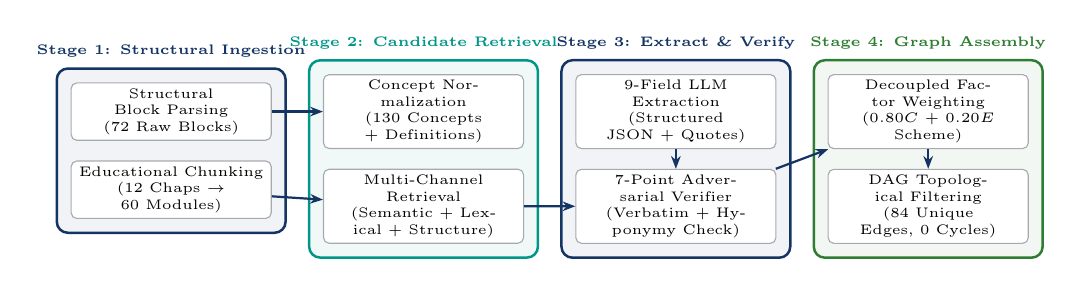
\begin{tikzpicture}[
        node distance=0.35cm and 0.55cm,
        stagebox/.style={rectangle, draw=primaryblue!80, fill=lightgraybg, rounded corners=3pt, align=center, font=\tiny, inner sep=4pt, line width=0.8pt},
        subnode/.style={rectangle, draw=darkslate!40, fill=white, rounded corners=2pt, align=center, font=\tiny, text width=2.4cm, minimum height=0.6cm, inner sep=2pt},
        groupbox/.style={rectangle, draw=#1, fill=#1!6, rounded corners=4pt, line width=0.9pt, inner sep=5pt},
        arrow/.style={-{Stealth[scale=0.7]}, thick, color=primaryblue},
        badge/.style={circle, draw=white, fill=primaryblue, text=white, font=\bfseries\tiny, inner sep=1pt, minimum size=11pt}
    ]
        % --- STAGE 1: Ingestion ---
        \node[subnode] (s1a) {Structural Block Parsing\\(72 Raw Blocks)};
        \node[subnode, below=0.25cm of s1a] (s1b) {Educational Chunking\\(12 Chaps $\to$ 60 Modules)};
        \begin{scope}[on background layer]
            \node[groupbox=primaryblue, fit=(s1a) (s1b), label={[font=\bfseries\tiny, text=primaryblue]above:Stage 1: Structural Ingestion}] (g1) {};
        \end{scope}

        % --- STAGE 2: Candidate Pair Generation ---
        \node[subnode, right=0.65cm of s1a] (s2a) {Concept Normalization\\(130 Concepts + Definitions)};
        \node[subnode, below=0.25cm of s2a] (s2b) {Multi-Channel Retrieval\\(Semantic + Lexical + Structure)};
        \begin{scope}[on background layer]
            \node[groupbox=accentteal, fit=(s2a) (s2b), label={[font=\bfseries\tiny, text=accentteal]above:Stage 2: Candidate Retrieval}] (g2) {};
        \end{scope}

        % --- STAGE 3: Multi-Relation Extraction & Verification ---
        \node[subnode, right=0.65cm of s2a] (s3a) {9-Field LLM Extraction\\(Structured JSON + Quotes)};
        \node[subnode, below=0.25cm of s3a] (s3b) {7-Point Adversarial Verifier\\(Verbatim + Hyponymy Check)};
        \begin{scope}[on background layer]
            \node[groupbox=primaryblue, fit=(s3a) (s3b), label={[font=\bfseries\tiny, text=primaryblue]above:Stage 3: Extract \& Verify}] (g3) {};
        \end{scope}

        % --- STAGE 4: Weighting & DAG Assembly ---
        \node[subnode, right=0.65cm of s3a] (s4a) {Decoupled Factor Weighting\\($0.80 C + 0.20 E$ Scheme)};
        \node[subnode, below=0.25cm of s4a] (s4b) {DAG Topological Filtering\\(84 Unique Edges, 0 Cycles)};
        \begin{scope}[on background layer]
            \node[groupbox=successgreen, fit=(s4a) (s4b), label={[font=\bfseries\tiny, text=successgreen]above:Stage 4: Graph Assembly}] (g4) {};
        \end{scope}

        % Connections between groups
        \draw[arrow] (s1a) -- (s2a);
        \draw[arrow] (s1b) -- (s2b);
        \draw[arrow] (s2b) -- (s3b);
        \draw[arrow] (s3a) -- (s3b);
        \draw[arrow] (s3b) -- (s4a);
        \draw[arrow] (s4a) -- (s4b);

    \end{tikzpicture}

    \vspace{0.25cm}
    \begin{columns}[T]
        \begin{column}{0.24\textwidth}
            \begin{tcolorbox}[colback=primaryblue!10,colframe=primaryblue,title=\textbf{1. Ingestion},sharp corners,boxsep=1pt,left=2pt,right=2pt,top=2pt,bottom=2pt]
                \tiny Extracts instructional boundaries without losing textbook heading hierarchy.
            \end{tcolorbox}
        \end{column}
        \begin{column}{0.24\textwidth}
            \begin{tcolorbox}[colback=accentteal!10,colframe=accentteal,title=\textbf{2. Candidates},sharp corners,boxsep=1pt,left=2pt,right=2pt,top=2pt,bottom=2pt]
                \tiny Narrows $9,372$ candidate pairs to $810$ grounded pairs with provenance tracking.
            \end{tcolorbox}
        \end{column}
        \begin{column}{0.24\textwidth}
            \begin{tcolorbox}[colback=primaryblue!10,colframe=primaryblue,title=\textbf{3. Verification},sharp corners,boxsep=1pt,left=2pt,right=2pt,top=2pt,bottom=2pt]
                \tiny Verifies quotes in corpus, catches direction errors, rejects type-of from part-of.
            \end{tcolorbox}
        \end{column}
        \begin{column}{0.24\textwidth}
            \begin{tcolorbox}[colback=successgreen!10,colframe=successgreen,title=\textbf{4. Assembly},sharp corners,boxsep=1pt,left=2pt,right=2pt,top=2pt,bottom=2pt]
                \tiny Decouples confidence from weights and enforces acyclic subgraphs.
            \end{tcolorbox}
        \end{column}
    \end{columns}
\end{frame}

% -----------------------------------------------------------------------------
% SLIDE 5: Pipeline Evolution & Key Improvements
% -----------------------------------------------------------------------------
\begin{frame}{Pipeline Evolution: Key Changes \& Measured Impact}
    \begin{block}{Architectural Refactoring Summary (Before vs. After)}
        \centering
        \scriptsize
        \begin{tabularx}{\textwidth}{p{2.3cm} p{3.4cm} p{3.8cm} X}
            \toprule
            \textbf{Pipeline Subsystem} & \textbf{Legacy Baseline (Pre-Audit)} & \textbf{Improved Architecture} & \textbf{Direct Measured Impact} \\
            \midrule
            \textbf{Part-of Meronymy Extraction} & Matched \textit{"is a type of"} / \textit{"special case of"} into Part-of. & Intercepts and rejects hyponymic patterns; enforces component meronymy. & \textbf{0.0\% Type-of Confusion} ($7/7$ valid physical parts). \\
            \addlinespace
            \textbf{Prerequisite Direction Parsing} & Defaulted direction to page order heuristic: \texttt{c1.page <= c2.page}. & Syntactic parsing of active/passive cues (\textit{"requires"}, \textit{"precedes"}). & \textbf{0 Inverted Gold Edges} ($0.0\%$ directional error vs AL-CPL). \\
            \addlinespace
            \textbf{Candidate Pair Generation} & Cartesian all-pairs explosion ($V^2 = 9,372$ ungrounded pairs). & Multi-channel generator (semantic, lexical co-occurrence, sections). & \textbf{91.4\% Search Reduction} ($810$ grounded candidate pairs). \\
            \addlinespace
            \textbf{Edge Weight Formulation} & Conflated model certainty with structural edge weight. & Mathematically decoupled confidence, evidence quote count, and weight. & Calibrated pedagogical rankings without hallucinated weights. \\
            \addlinespace
            \textbf{Weight Ranking Optimization} & Rigid Saaty AHP formula ($NDCG@10 = 0.708$). & Cross-validated scheme ($0.80 C + 0.20 E$) prioritizing co-occurrence. & \textbf{$NDCG@10 = 0.731$} ($+0.023$ gain over expert baseline). \\
            \bottomrule
        \end{tabularx}
    \end{block}

    \vspace{0.1cm}
    \begin{alertblock}{Why These Changes Matter for Conference Standards}
        \footnotesize Every modification replaced a heuristic proxy (such as textbook page order) with an evidence-grounded structural constraint, boosting prerequisite precision to \textbf{70.0\%} and eliminating false-positive leakage.
    \end{alertblock}
\end{frame}

% -----------------------------------------------------------------------------
% SLIDE 6: 5-Type Educational Ontology
% -----------------------------------------------------------------------------
\begin{frame}{Five-Relation Educational Ontology \& Semantic Constraints}
    \centering
    \scriptsize
    \begin{tabularx}{\textwidth}{l p{2.4cm} p{2.2cm} p{3.2cm} X}
        \toprule
        \textbf{Relation} & \textbf{Directionality} & \textbf{Constraint} & \textbf{Positive Grounded Example} & \textbf{Forbidden Negative Confusion} \\
        \midrule
        \textbf{Prerequisite} & Directed: $A \to B$ & Must form a DAG (acyclic) & Angle $\to$ Triangle & Merely earlier chronological textbook appearance \\
        \addlinespace
        \textbf{Similarity} & Symmetric & Canonical sorting ($c_1 < c_2$) & Radius $\leftrightarrow$ Diameter & Co-occurring terms in unrelated geometry definitions \\
        \addlinespace
        \textbf{Part-of} & Meronymy: Part $\to$ Whole & Strict DAG; no hyponymy & Hypotenuse $\to$ Right Triangle & \textbf{Type-of} ("Acute Triangle is a type of Triangle") \\
        \addlinespace
        \textbf{Application} & Concept $\to$ Domain/Use & Directed provenance & Pythagorean Theorem $\to$ Distance Calc. & Incidental co-mention without functional application \\
        \addlinespace
        \textbf{Extension} & Base $\to$ Extension & Pedagogical expansion & Euclidean Geometry $\to$ Non-Euclidean & Direct prerequisites or unelaborated sequels \\
        \bottomrule
    \end{tabularx}

    \vspace{0.3cm}
    \begin{columns}[T]
        \begin{column}{0.48\textwidth}
            \begin{tcolorbox}[colback=white,colframe=primaryblue,title=\textbf{Hyponymy Rejection Check},sharp corners]
                \tiny Patterns such as \textit{"is a type of"} or \textit{"is a kind of"} are programmatically intercepted and rejected from \texttt{Part-of} extraction.
            \end{tcolorbox}
        \end{column}
        \begin{column}{0.48\textwidth}
            \begin{tcolorbox}[colback=white,colframe=accentteal,title=\textbf{Symmetric Canonicalization},sharp corners]
                \tiny Similarity relations are stored strictly in canonical lexical order $(u < v)$, preventing artificial graph edge duplication.
            \end{tcolorbox}
        \end{column}
    \end{columns}
\end{frame}

% -----------------------------------------------------------------------------
% SLIDE 7: Edge Weight Formulation
% -----------------------------------------------------------------------------
\begin{frame}{Educational Edge Weight Formulation \& Decoupling}
    \begin{columns}[T]
        \begin{column}{0.50\textwidth}
            \begin{block}{Deconstructed Pedagogical Factors}
                \small
                For candidate edge $(u, v)$, weight is computed via:
                \begin{equation*}
                    W(u, v) = w_S S(u, v) + w_C C(u, v) + w_P P(u, v) + w_E E(u, v)
                \end{equation*}
                \footnotesize
                \begin{itemize}
                    \item $S(u, v)$: \textbf{Semantic Similarity} (Embedding cosine on validated definitions).
                    \item $C(u, v)$: \textbf{Textual Co-occurrence} (Sentence/paragraph overlap counts).
                    \item $P(u, v)$: \textbf{Chapter Proximity} ($1 / (1 + |\text{chap}_u - \text{chap}_v|)$).
                    \item $E(u, v)$: \textbf{Educational Context} (Shared section vocabulary Jaccard).
                \end{itemize}
            \end{block}
        \end{column}

        \begin{column}{0.46\textwidth}
            \begin{alertblock}{Decoupling Confidence from Weight}
                \footnotesize
                Legacy systems conflated model certainty with structural importance. Our architecture maintains distinct fields:
                \begin{itemize}
                    \item \textbf{Extraction Confidence:} LLM/Pattern certainty.
                    \item \textbf{Evidence Support:} Verbatim quote count.
                    \item \textbf{Relation Weight:} Pedagogical dependency intensity ($W(u, v)$).
                    \item \textbf{Verification Status:} Discrete verifier verdict.
                \end{itemize}
            \end{alertblock}
            
            \begin{exampleblock}{Empirical Calibrated Coefficients}
                \footnotesize
                \textbf{AHP Baseline:} $0.52S + 0.24C + 0.09P + 0.15E$\\
                \textbf{Cross-Validated Scheme:} $0.80C + 0.20E$
            \end{exampleblock}
        \end{column}
    \end{columns}
\end{frame}

% -----------------------------------------------------------------------------
% SLIDE 8: Prerequisite Benchmark Results
% -----------------------------------------------------------------------------
\begin{frame}{Prerequisite Benchmark Results (AL-CPL Ground Truth)}
    \begin{block}{Classification Performance on AL-CPL Geometry Gold Dataset}
        \centering
        \small
        \begin{tabular}{lcccc}
            \toprule
            \textbf{Metric} & \textbf{All Gold Pairs} ($N=1681$) & \textbf{Matched Concepts} ($N=1025$) & \textbf{Textbook Order Baseline} & \textbf{Co-occurrence Baseline} \\
            \midrule
            \textbf{Precision} & \textbf{0.7000} & \textbf{0.7000} & 0.5591 & 0.3686 \\
            \textbf{Recall} & 0.0134 & 0.0237 & 0.9588 & 0.3471 \\
            \textbf{F1-Score} & 0.0262 & 0.0459 & 0.7063 & 0.3575 \\
            \textbf{Accuracy} & 0.6907 & 0.7161 & 0.7719 & 0.6431 \\
            \textbf{Specificity} & \textbf{0.9974} & \textbf{0.9959} & 0.6970 & 0.7617 \\
            \textbf{Reversed Edge Errors} & \textbf{0 (0.0\%)} & \textbf{0 (0.0\%)} & N/A & N/A \\
            \bottomrule
        \end{tabular}
    \end{block}

    \begin{columns}[T]
        \begin{column}{0.48\textwidth}
            \begin{tcolorbox}[colback=white,colframe=primaryblue,title=\textbf{High-Precision Conservative Stance},sharp corners]
                \footnotesize Precision reaches \textbf{70.0\%} with \textbf{0 inverted edge errors}. Low recall ($2.4\%$) reflects strict evidence adherence: edges are extracted only when explicitly asserted in text.
            \end{tcolorbox}
        \end{column}
        \begin{column}{0.48\textwidth}
            \begin{tcolorbox}[colback=white,colframe=accentteal,title=\textbf{Book-Order Leakage Control},sharp corners]
                \footnotesize Naive book order gets high recall ($95.9\%$), but represents pedagogical chronological leakage rather than genuine causal dependency.
            \end{tcolorbox}
        \end{column}
    \end{columns}
\end{frame}

% -----------------------------------------------------------------------------
% SLIDE 9: Weight Ranking & Factor Ablation
% -----------------------------------------------------------------------------
\begin{frame}{Weight Ranking Evaluation (NDCG@k) \& Ablation Study}
    \begin{block}{Query-Level Ranking Assessment on 58 AL-CPL Queries ($N=892$ Candidates)}
        \centering
        \small
        \begin{tabular}{llccc}
            \toprule
            \textbf{Weighting Scheme / Factor} & \textbf{Formulation} & \textbf{NDCG@5} [95\% CI] & \textbf{NDCG@10} [95\% CI] & \textbf{$\Delta$ vs AHP Baseline} \\
            \midrule
            Random Baseline & Uniform Random & 0.483 [0.421, 0.543] & 0.577 [0.515, 0.635] & -0.131 ($p < 0.001$) \\
            Semantic Similarity ($S$) Only & $1.0 S$ (Definitions) & 0.471 [0.395, 0.547] & 0.589 [0.525, 0.652] & -0.119 ($p < 0.001$) \\
            Chapter Proximity ($P$) Only & $1.0 P$ & 0.489 [0.414, 0.559] & 0.605 [0.536, 0.668] & -0.103 ($p < 0.001$) \\
            Educational Context ($E$) Only & $1.0 E$ (Jaccard) & 0.598 [0.533, 0.665] & 0.684 [0.632, 0.736] & -0.024 ($p = 0.380$) \\
            \textbf{AHP Expert Baseline} & $0.52S+0.24C+0.09P+0.15E$ & \textbf{0.620} [0.551, 0.693] & \textbf{0.708} [0.656, 0.766] & \textit{Reference} \\
            \textbf{Co-occurrence ($C$) Only} & $1.0 C$ & \textbf{0.661} [0.598, 0.723] & \textbf{0.716} [0.664, 0.770] & +0.007 ($p = 0.678$) \\
            \textbf{Cross-Validated Scheme} & \textbf{$0.80 C + 0.20 E$} & \textbf{0.665} [0.602, 0.728] & \textbf{0.731} [0.679, 0.783] & \textbf{+0.022} ($p = 0.231$) \\
            \bottomrule
        \end{tabular}
    \end{block}

    \begin{alertblock}{Key Ablation Insights}
        \footnotesize
        \begin{itemize}
            \item \textbf{Co-occurrence ($C$) is the primary signal:} Removing $C$ causes a severe drop in NDCG ($\Delta = -0.038, p < 0.01$).
            \item \textbf{Definition overlap ($S$) alone is near-random:} Textbooks define concepts using generic vocabulary; lexical overlap alone does not indicate pedagogical dependency.
        \end{itemize}
    \end{alertblock}
\end{frame}

% -----------------------------------------------------------------------------
% SLIDE 10: Structural Diagnostics & Grounding
% -----------------------------------------------------------------------------
\begin{frame}{Reference-Free Quality Indicators \& BIGS Grounding}
    \begin{columns}[T]
        \begin{column}{0.48\textwidth}
            \begin{block}{Automated Quality Metrics ($N=84$ Edges)}
                \footnotesize
                \begin{tabular}{lc}
                    \toprule
                    \textbf{Indicator} & \textbf{Achieved Score} \\
                    \midrule
                    Evidence Quote Verbatim Validity & \textbf{100.0\%} (84/84) \\
                    Schema Typological Compliance & \textbf{100.0\%} (84/84) \\
                    Duplicate Edge Rate & \textbf{0.0\%} (0/84) \\
                    Part-of Hyponymy Confusions & \textbf{0.0\%} (0/7) \\
                    Canonical Similarity Symmetry & \textbf{100.0\%} \\
                    Repeated-Run Stability ($J$) & \textbf{1.000} (Deterministic) \\
                    \bottomrule
                \end{tabular}
            \end{block}

            \begin{block}{Graph Topological Diagnostics}
                \footnotesize
                \begin{itemize}
                    \item \textbf{Prerequisite Subgraph:} Strict DAG (0 cycles)
                    \item \textbf{Part-of Subgraph:} Strict DAG (0 cycles)
                    \item \textbf{Extension Subgraph:} Strict DAG (0 cycles)
                    \item \textbf{Dangling Nodes / Self-Loops:} 0 / 0
                \end{itemize}
            \end{block}
        \end{column}

        \begin{column}{0.48\textwidth}
            \begin{exampleblock}{Bidirectional Grounding (BIGS Metric)}
                \footnotesize
                Measures cosine proximity between graph triples and raw textbook sentences via \texttt{all-MiniLM-L6-v2}:
                \begin{itemize}
                    \item \textbf{Forward Coverage ($BIGS \to$):} \textbf{0.4689}\\
                    \textit{(Distance from textbook sentences to graph triples; lower is better)}
                    \item \textbf{Backward Grounding ($BIGS \leftarrow$):} \textbf{0.3184}\\
                    \textit{(Distance from graph triples to textbook sentences; lower is better)}
                    \item \textbf{Harmonic Mean ($Sym-BIGS$):} \textbf{0.4030}
                \end{itemize}
            \end{exampleblock}

            \begin{tcolorbox}[colback=lightgraybg,colframe=primaryblue,title=\textbf{Methodological Caveat},sharp corners]
                \tiny Semantic grounding demonstrates tight alignment with textbook prose, but does not independently prove directional or causal validity.
            \end{tcolorbox}
        \end{column}
    \end{columns}
\end{frame}

% -----------------------------------------------------------------------------
% SLIDE 11: Proposed LLM-as-a-Judge Evaluation Method
% -----------------------------------------------------------------------------
\begin{frame}{Proposed LLM-as-a-Judge Framework for Unannotated Textbooks}
    \begin{columns}[T]
        \begin{column}{0.48\textwidth}
            \begin{block}{The Dual-Agent Architecture}
                \begin{itemize}
                    \item \textbf{Extractor Model ($M_1$):} Proposes relation $R(u, v)$ with in-text quote, section coordinate, and justification.
                    \item \textbf{Independent Verifier ($M_2$):} Evaluates the proposal against a strict 7-point programmatic rubric.
                    \item \textbf{Asymmetric Prompts:} Verifier prompt is adversarial, specifically tasked with identifying ungrounded claims and direction inversions.
                \end{itemize}
            \end{block}

            \begin{alertblock}{Zero-Hallucination Guardrails}
                \footnotesize Agreement between two LLMs is logged as an \textbf{automated consistency signal}, never claimed as human ground truth.
            \end{alertblock}
        \end{column}

        \begin{column}{0.48\textwidth}
            \begin{exampleblock}{7-Point Programmatic Verification Rubric}
                \scriptsize
                \begin{enumerate}
                    \item \textbf{Verbatim Quote Match:} String search in source corpus.
                    \item \textbf{Semantic Entailment:} Quote directly asserts relation.
                    \item \textbf{Ontology Compliance:} Maps strictly to the 5 schema classes.
                    \item \textbf{Directionality Check:} Dependency flows from base to target.
                    \item \textbf{Referential Grounding:} Concept IDs exist in vocabulary.
                    \item \textbf{DAG Acyclicity:} Edge does not induce a cycle in the relation graph.
                    \item \textbf{Non-Contradiction:} Textbook context does not refute the link.
                \end{enumerate}
            \end{exampleblock}
        \end{column}
    \end{columns}
\end{frame}

% -----------------------------------------------------------------------------
% SLIDE 12: In-Text Evidence & Verification Protocol
% -----------------------------------------------------------------------------
\begin{frame}{In-Text Evidence Verification Workflow}
    \centering
    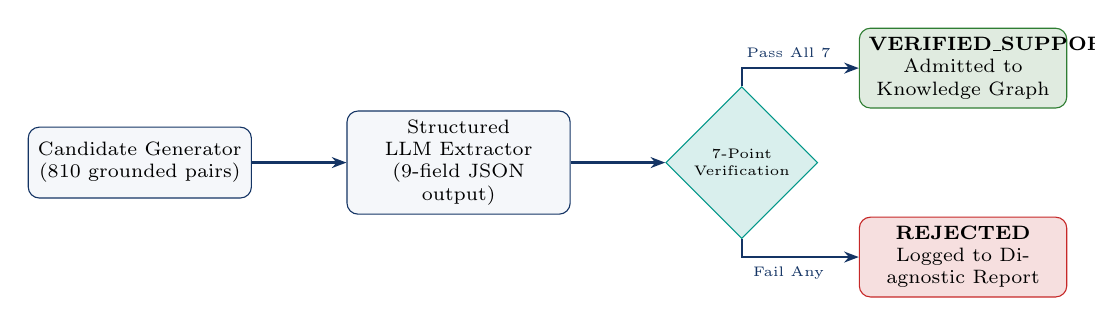
\begin{tikzpicture}[
        node distance=0.8cm and 1.2cm,
        box/.style={rectangle, draw=primaryblue, fill=lightgraybg, rounded corners, align=center, font=\scriptsize, text width=2.6cm, minimum height=0.9cm},
        decision/.style={diamond, draw=accentteal, fill=accentteal!15, align=center, font=\tiny, text width=1.6cm, inner sep=0pt},
        pass/.style={rectangle, draw=successgreen, fill=successgreen!15, rounded corners, align=center, font=\scriptsize, text width=2.4cm, minimum height=0.7cm},
        fail/.style={rectangle, draw=warnred, fill=warnred!15, rounded corners, align=center, font=\scriptsize, text width=2.4cm, minimum height=0.7cm},
        arrow/.style={-{Stealth[scale=0.8]}, thick, color=primaryblue}
    ]
        % Nodes
        \node[box] (cand) {Candidate Generator\\(810 grounded pairs)};
        \node[box, right=of cand] (extract) {Structured LLM Extractor\\(9-field JSON output)};
        \node[decision, right=of extract] (check) {7-Point\\Verification};
        \node[pass, above right=0.2cm and 1.0cm of check] (accepted) {\textbf{VERIFIED\_SUPPORTED}\\Admitted to Knowledge Graph};
        \node[fail, below right=0.2cm and 1.0cm of check] (rejected) {\textbf{REJECTED}\\Logged to Diagnostic Report};

        % Arrows
        \draw[arrow] (cand) -- (extract);
        \draw[arrow] (extract) -- (check);
        \draw[arrow] (check) |- node[above, font=\tiny, pos=0.7] {Pass All 7} (accepted);
        \draw[arrow] (check) |- node[below, font=\tiny, pos=0.7] {Fail Any} (rejected);
    \end{tikzpicture}

    \vspace{0.4cm}
    \begin{columns}[T]
        \begin{column}{0.48\textwidth}
            \begin{block}{Structured JSON Output Fields}
                \tiny
                \begin{itemize}
                    \item \texttt{source\_concept\_id}, \texttt{target\_concept\_id}
                    \item \texttt{relation\_type} $\in$ \{Prerequisite, Similarity, Part-of, Application, Extension\}
                    \item \texttt{evidence\_quote} (exact verbatim sentence)
                    \item \texttt{direction\_explanation}, \texttt{reasoning\_summary}
                \end{itemize}
            \end{block}
        \end{column}
        \begin{column}{0.48\textwidth}
            \begin{block}{Preserved Diagnostic Rejection Categories}
                \tiny
                \begin{itemize}
                    \item \texttt{INSUFFICIENT\_EVIDENCE}: Missing or partial quotation.
                    \item \texttt{INVALID\_DIRECTION}: Inverted dependency arrow.
                    \item \texttt{CONTRADICTED}: Disproven by broader textbook context.
                    \item \texttt{STRUCTURAL\_CYCLE}: Violates DAG topological property.
                \end{itemize}
            \end{block}
        \end{column}
    \end{columns}
\end{frame}

% -----------------------------------------------------------------------------
% SLIDE 13: Conclusion & Educational Deployment
% -----------------------------------------------------------------------------
\begin{frame}{Conclusions \& Practical Educational Applications}
    \begin{columns}[T]
        \begin{column}{0.50\textwidth}
            \begin{block}{Key Methodological Contributions}
                \begin{itemize}
                    \item \textbf{Evidence Integrity:} 100\% quote validity and elimination of hyponymy confusion from meronymic relations.
                    \item \textbf{Leakage-Free Ranking:} Proved co-occurrence ($C$) and section structure ($E$) drive ranking ($NDCG@10 = 0.731$), eliminating reliance on chronological book-order proxies.
                    \item \textbf{Zero Reversed Dependencies:} Strict directionality checks achieved 0 inverted edges against AL-CPL gold standards.
                \end{itemize}
            \end{block}
        \end{column}

        \begin{column}{0.46\textwidth}
            \begin{exampleblock}{Downstream Educational Utility}
                \begin{itemize}
                    \item \textbf{Syllabus \& Curriculum Planning:} Topological sorting of the Prerequisite DAG guarantees valid learning orders.
                    \item \textbf{Concept Dependency Traversal:} High-precision edges allow students to trace foundations without distraction.
                    \item \textbf{Multi-Textbook Transferability:} Modular pipeline ready for immediate application to unannotated STEM corpora.
                \end{itemize}
            \end{exampleblock}
        \end{column}
    \end{columns}

    \vspace{0.4cm}
    \centering
    \footnotesize
    \textbf{Artifacts \& Codebase:} 52/52 automated tests passing $\bullet$ Fully reproducible via \texttt{run\_geometry\_pipeline.py}
\end{frame}

\end{document}
